% This is a Basic Assignment Paper but with like Code and stuff allowed in it, there is also url, hyperlinks from contents included. 

\documentclass[11pt]{article}

% Preamble

\usepackage[margin=1in]{geometry}
\usepackage{amsfonts, amsmath, amssymb}
\usepackage{fancyhdr, float, graphicx}
\usepackage[utf8]{inputenc} % Required for inputting international characters
\usepackage[T1]{fontenc} % Output font encoding for international characters
\usepackage{fouriernc} % Use the New Century Schoolbook font
\usepackage[nottoc, notlot, notlof]{tocbibind}
\usepackage{listings}
\usepackage{xcolor}
\usepackage{blindtext}
\usepackage{hyperref}
\usepackage{booktabs}
\hypersetup{
    colorlinks=true,
    linkcolor=black,
    filecolor=magenta,      
    urlcolor=cyan,
    pdfpagemode=FullScreen,
    }

\definecolor{codegreen}{rgb}{0,0.6,0}
\definecolor{codegray}{rgb}{0.5,0.5,0.5}
\definecolor{codepurple}{rgb}{0.58,0,0.82}
\definecolor{backcolour}{rgb}{0.95,0.95,0.92}

\lstdefinestyle{mystyle}{
    backgroundcolor=\color{backcolour},   
    commentstyle=\color{codegreen},
    keywordstyle=\color{magenta},
    numberstyle=\tiny\color{codegray},
    stringstyle=\color{codepurple},
    basicstyle=\ttfamily\footnotesize,
    breakatwhitespace=false,         
    breaklines=true,                 
    captionpos=b,                    
    keepspaces=true,                 
    numbers=left,                    
    numbersep=5pt,                  
    showspaces=false,                
    showstringspaces=false,
    showtabs=false,                  
    tabsize=2
}

\lstset{style=mystyle}

% Header and Footer
\pagestyle{fancy}
\fancyhead{}
\fancyfoot{}
\fancyhead[L]{\textit{\Large{Advanced Data Structures - Assignment 7}}}
%\fancyhead[R]{\textit{something}}
\fancyfoot[C]{\thepage}
\renewcommand{\footrulewidth}{1pt}



% Other Doc Editing
% \parindent 0ex
%\renewcommand{\baselinestretch}{1.5}

\begin{document}

\begin{titlepage}
    \centering

    %---------------------------NAMES-------------------------------

    \huge\textsc{
        MIT World Peace University
    }\\

    \vspace{0.75\baselineskip} % space after Uni Name

    \LARGE{
        Advanced Data Structures\\
        Second Year B. Tech, Semester 4
    }

    \vfill % space after Sub Name

    %--------------------------TITLE-------------------------------

    \rule{\textwidth}{1.6pt}\vspace*{-\baselineskip}\vspace*{2pt}
    \rule{\textwidth}{0.6pt}
    \vspace{0.75\baselineskip} % Whitespace above the title



    \huge{\textsc{
            Implementation of Heap as a Data Structure
        }} \\



    \vspace{0.5\baselineskip} % Whitespace below the title
    \rule{\textwidth}{0.6pt}\vspace*{-\baselineskip}\vspace*{2.8pt}
    \rule{\textwidth}{1.6pt}

    \vspace{1\baselineskip} % Whitespace after the title block

    %--------------------------SUBTITLE --------------------------	

    \LARGE\textsc{
        Assignment No. 7
    } % Subtitle or further description
    \vfill

    %--------------------------AUTHOR-------------------------------

    Prepared By
    \vspace{0.5\baselineskip} % Whitespace before the editors

    \Large{
        Krishnaraj Thadesar \\
        Cyber Security and Forensics\\
        Batch A1, PA 20
    }


    \vspace{0.5\baselineskip} % Whitespace below the editor list
    \today

\end{titlepage}

\tableofcontents
\thispagestyle{empty}
\clearpage

\setcounter{page}{1}

\section{Objectives}
\begin{enumerate}
    \item To study the concept of heap
    \item To study different types of heap and their algorithms
\end{enumerate}

\section{Problem Statement}
\textit{Read the marks obtained by students of second year in an online examination of
    particular subject. Find out maximum and minimum marks obtained in that subject. Use
    heap data structure and Heap sort.}
\section{Theory}

\subsection{Heap}

A heap is a specialized tree-based data structure that satisfies the heap property. The heap property is a condition where each node in the tree is greater than or equal to (in a max heap) or less than or equal to (in a min heap) its children. The root node of the heap is the maximum (or minimum) element in a max (or min) heap.

Heaps are often used to implement priority queues, where elements are extracted in order of priority. For example, in a hospital, patients with the most urgent medical needs are given the highest priority for treatment. A priority queue based on a heap can efficiently manage the order of patients by storing their priority level (e.g., critical, urgent, or routine) in each node and maintaining the heap property.

\begin{figure}[H]
    \centering
    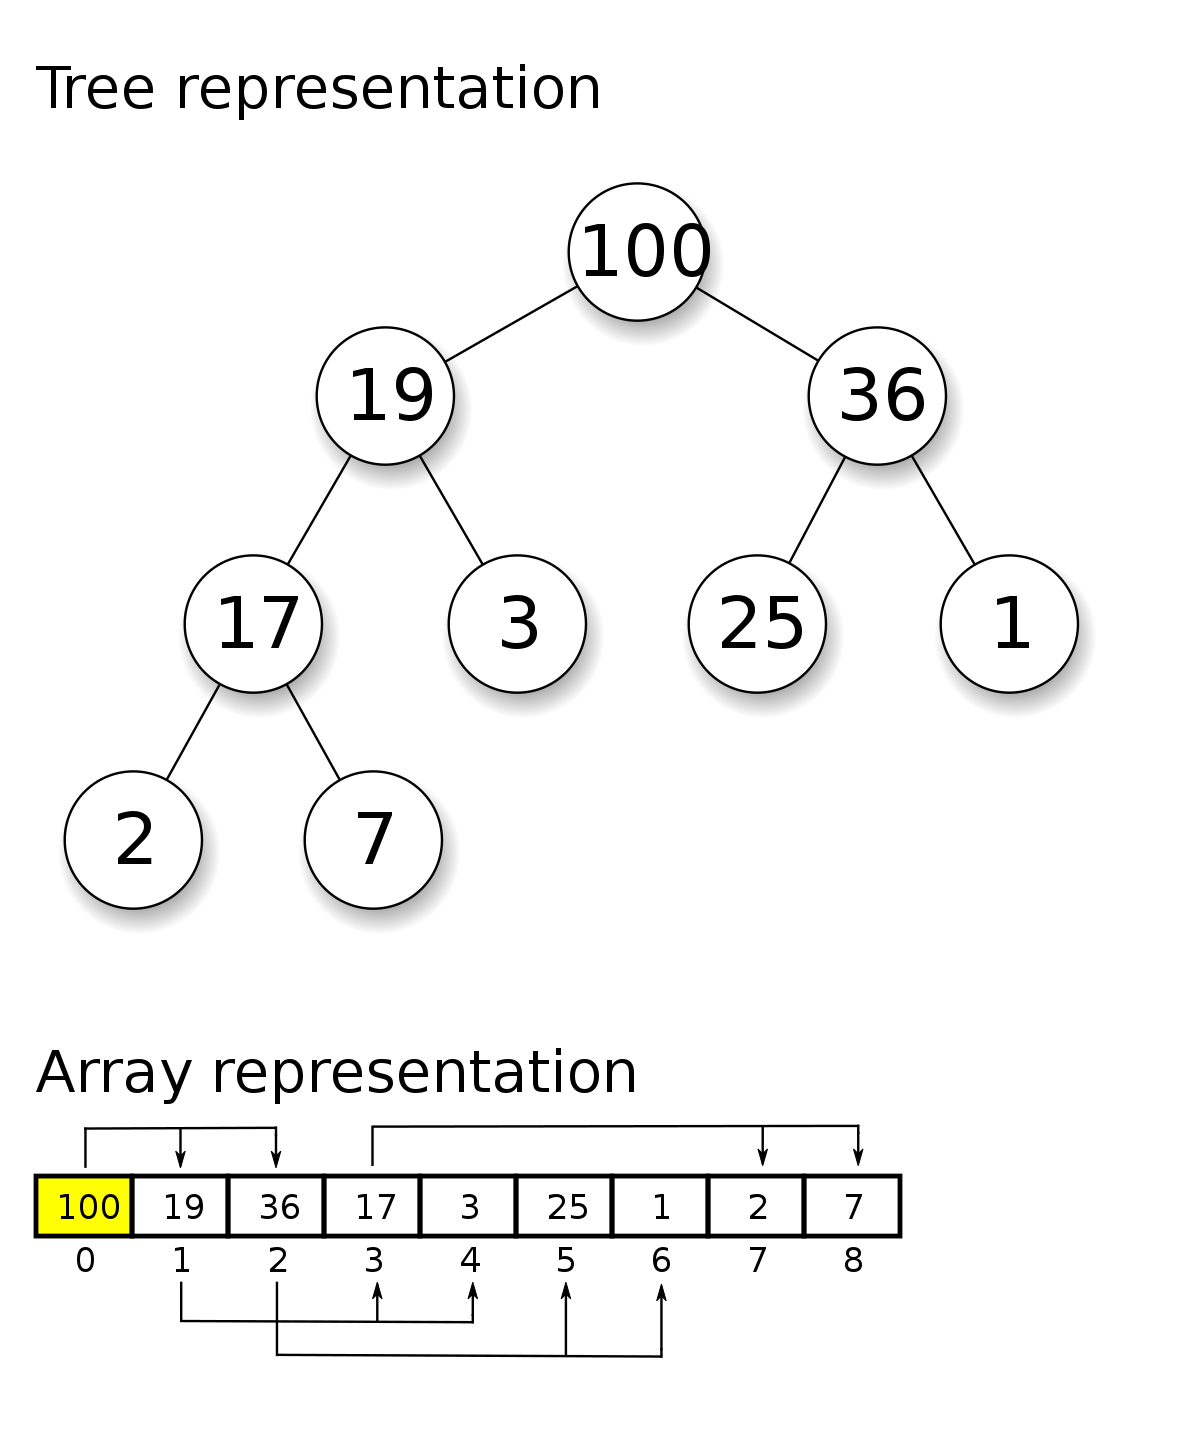
\includegraphics[width=.45\textwidth]{1200px-Max-Heap-new.svg.png}
    \caption{}
\end{figure}


\subsection{Types of Heaps}

There are two main types of heaps: max heaps and min heaps. In a max heap, the maximum element is always stored at the root, and every node is greater than or equal to its children. In a min heap, the minimum element is stored at the root, and every node is less than or equal to its children.

Both types of heaps have their own advantages and use cases. Max heaps are often used to implement priority queues, where the highest priority element needs to be extracted first. Min heaps are often used in algorithms such as Dijkstra's shortest path algorithm, where the minimum distance to a vertex needs to be determined.

\begin{figure}[H]
    \centering
    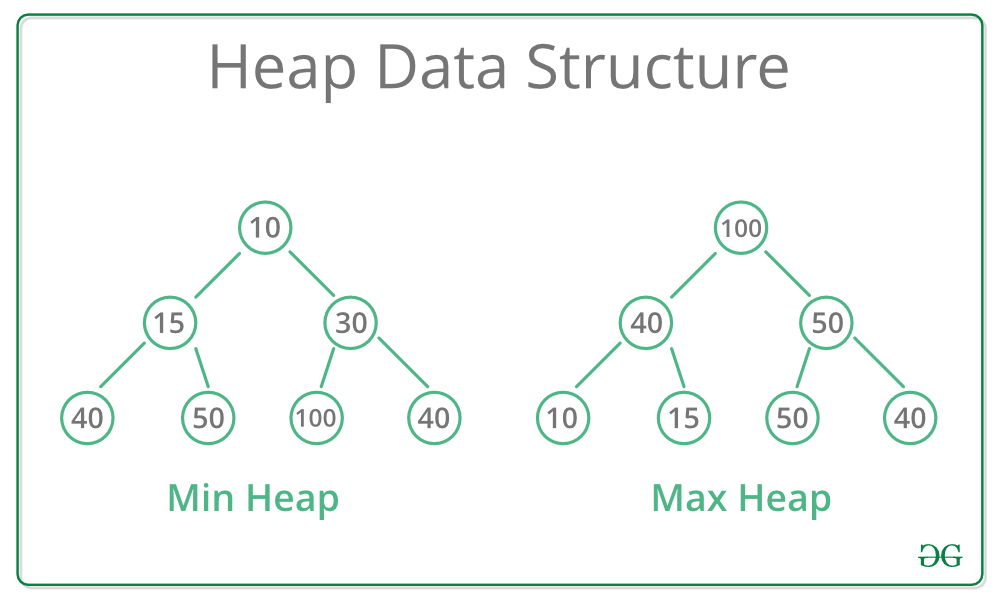
\includegraphics[width=.45\textwidth]{MinHeapAndMaxHeap1.png}
    \caption{Min Heap and Max Heap}
\end{figure}

\subsection{Construction of heaps}

Heaps can be constructed using a variety of algorithms, including the bottom-up construction algorithm and the top-down construction algorithm. The bottom-up construction algorithm starts with a partially ordered set of elements and iteratively adds elements to the heap in a way that maintains the heap property. The top-down construction algorithm starts with an empty heap and iteratively adds elements to the heap in a way that maintains the heap property.

Regardless of the algorithm used, the construction of a heap takes O(n) time, where n is the number of elements in the heap. This is because each element must be inserted into the heap and the heap property must be maintained at each step.

\begin{figure}[H]
    \centering
    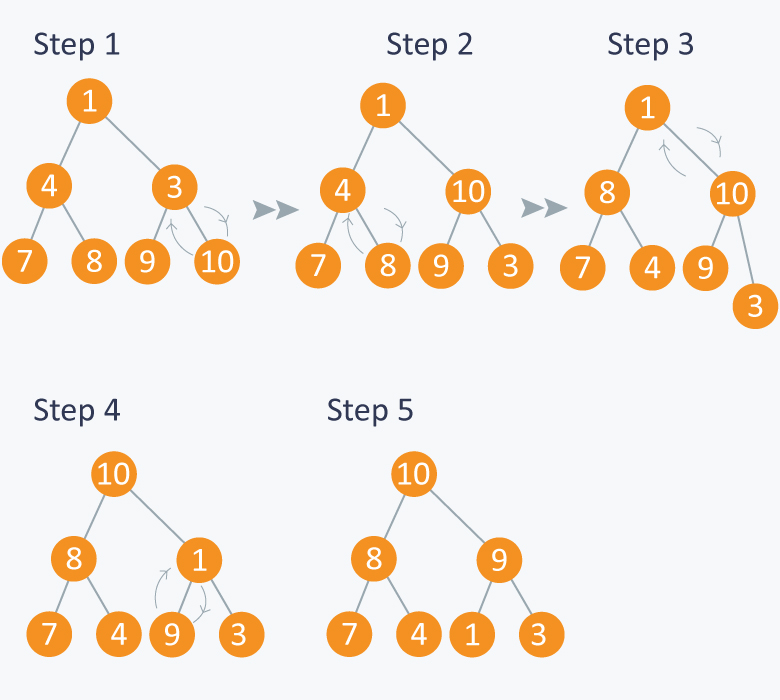
\includegraphics[width=.45\textwidth]{af2e932.jpg}
    \caption{}
\end{figure}

\subsection{Data Structures Used for Heap Constructions}

The most common data structure used for heap construction is an array. In an array-based heap, the elements are stored in an array in a way that maintains the heap property. The root element is stored at index 0, and the children of a node at index i are stored at indices 2i+1 and 2i+2.

Linked lists can also be used to implement heaps, but they are less commonly used due to their higher overhead.

\subsection{Time and Space Complexities Associated with Heap}

The time complexity of heap operations depends on the height of the heap, which is O(log n) for a heap with n elements. The space complexity of a heap is O(n), where n is the number of elements in the heap.

Inserting an element into a heap takes O(log n) time, as the element must be inserted at the bottom of the heap and then sifted up to maintain the heap property. Similarly, extracting the maximum (or minimum) element from a heap takes O(log n) time, as the root element must be removed and then the heap must be reorganized to maintain the heap property.

Heap operations are generally more efficient than operations on other data structures such as arrays or linked lists, particularly for large datasets. However, they can be less efficient than other data structures for small datasets due to the overhead associated with maintaining the heap property.

\subsection{Heap Vs Binary Search Trees}

Heaps are often compared to binary search trees (BSTs), another tree-based data structure. However, heaps are not as efficient as BSTs for all operations. For example, searching for an element in a heap takes O(n) time, as each element must be searched in the worst case. In contrast, searching for an element in a BST takes O(log n) time, as the search can be narrowed down to a single subtree.

However, heaps are more efficient than BSTs for operations such as finding the maximum (or minimum) element, as the root element is always the maximum (or minimum) element in a heap. In contrast, finding the maximum (or minimum) element in a BST takes O(log n) time, as the maximum (or minimum) element may be located at the bottom of the tree.

\subsection{Applications of Heap}

Heaps are often used to implement priority queues, where elements are extracted in order of priority. For example, in a hospital, patients with the most urgent medical needs are given the highest priority for treatment. A priority queue based on a heap can efficiently manage the order of patients by storing their priority level (e.g., critical, urgent, or routine) in each node and maintaining the heap property.

Heaps are also used in algorithms such as Dijkstra's shortest path algorithm, where the minimum distance to a vertex needs to be determined. In this case, the heap stores the vertices that have not yet been visited, and the minimum distance to each vertex is stored in each node. The heap property is maintained by updating the minimum distance to each vertex as the algorithm progresses.


\section{Platform}
\textbf{\textbf{Operating System}}: Arch Linux x86-64 \\
\textbf{\textbf{IDEs or Text Editors Used}}: Visual Studio Code\\
\textbf{\textbf{Compilers} }: g++ and gcc on linux for C++\\

\section{Test Conditions}
\begin{enumerate}
    \item Input min 10 elements.
    \item Display Max and Min Heap
    \item Find Maximum and Minimum marks obtained in a particular subject.
\end{enumerate}

\section{Input and Output}
\begin{enumerate}
    \item The minimum cost of the spanning tree.
\end{enumerate}

\section{Pseudo Code}
\subsubsection*{Pseudo Code for Creation of Min and Max Heap}
\begin{lstlisting}[language=c++]
CreateMaxHeap(array)
    for i from n/2 down to 1 do:
        MaxHeapify(array, i, n)

CreateMinHeap(array)
    for i from n/2 down to 1 do:
        MinHeapify(array, i, n)

\end{lstlisting}
\subsubsection*{Pseudo Code for Heapify function}
\begin{lstlisting}[language=c++]
MaxHeapify(array, i, n)
    left = 2i
    right = 2i + 1
    largest = i
    
    if left <= n and array[left] > array[largest] then:
        largest = left
    if right <= n and array[right] > array[largest] then:
        largest = right
    if largest != i then:
        swap(array[i], array[largest])
        MaxHeapify(array, largest, n)

MinHeapify(array, i, n)
    left = 2i
    right = 2i + 1
    smallest = i
    
    if left <= n and array[left] < array[smallest] then:
        smallest = left
    if right <= n and array[right] < array[smallest] then:
        smallest = right
    if smallest != i then:
        swap(array[i], array[smallest])
        MinHeapify(array, smallest, n)

\end{lstlisting}


\section{Time Complexity}

\subsection{Min and Max Heap Creation}
\begin{itemize}
    \item \textbf{Time Complexity:} \[ O(n\log(n))\]
    \item \textbf{Space Complexity:} \[ O(n) \]
\end{itemize}

\subsection{Min or Max Heap Traversal}

\begin{itemize}
    \item \textbf{Time Complexity:} \[ O(n\log(n))\]
    \item \textbf{Space Complexity:} \[ O(n) \]
\end{itemize}

\subsection{Heap Sort}

\begin{itemize}
    \item \textbf{Time Complexity:} \[ O(n\log(n))\]
    \item \textbf{Space Complexity:} \[ O(n) \]
\end{itemize}

\section{Searching in Heap}

\begin{itemize}
    \item \textbf{Time Complexity:} \[ O(n) \]
\end{itemize}

\section{Code}

\subsection{Program}
\lstinputlisting[language=C++]{../Programs/Assignment_7.cpp}

\lstinputlisting[]{../Programs/Assignment_7_output.txt}

\section{Conclusion}
Thus, we have understood the importance and use of Heaps as a Data structure, and how they are better and more efficient than Binary Search Trees. We have also understood the working of Heap Sort and how it is implemented.

\clearpage

\section{FAQ}
\begin{enumerate}
    \item \textbf{Discuss with suitable example for heap sort?}\\
          Heap sort is a comparison-based sorting algorithm that works by first organizing the data to be sorted into a binary heap. The heap is then repeatedly reduced to a sorted array by extracting the largest element from the heap and inserting it into the output array. The heap is reconstructed after each extraction.

          An example of heap sort can be shown using the following array of numbers:

          [12, 11, 13, 5, 6, 7]

          First, we build a max heap from the given array. The max heap is a binary tree where the parent node is greater than or equal to its children. After building the max heap, the array becomes:

          [13, 11, 12, 5, 6, 7]

          The first element of the array is the largest number in the heap, so we move it to the end of the array and reduce the heap size by one. The array now becomes:

          [7, 11, 12, 5, 6, 13]

          We then rebuild the max heap from the remaining elements and repeat the process until the heap is empty. The sorted array is obtained by repeatedly extracting the maximum element from the heap and appending it to the output array. The final sorted array is:

          [5, 6, 7, 11, 12, 13]


    \item \textbf{Compute the time complexity of heap sort?}\\
          The time complexity of heap sort is O(n log n) in the worst case, where n is the number of elements to be sorted. This is because the max heap can be built in O(n) time and each extraction from the heap takes O(log n) time. Therefore, the total time complexity of heap sort is O(n log n). Heap sort is efficient for large datasets and is a good choice when a stable sort is not required.
\end{enumerate}

\end{document}